\documentclass{article}

\usepackage{times}
\usepackage{geometry}
\geometry{a4paper,left=0.6cm,right=0.7cm,top=1cm,bottom=1cm,columnsep=0.8cm}

\usepackage{fontawesome}
\usepackage[hidelinks]{hyperref}
\usepackage{multicol,paracol,tikz,hyphsubst,moresize,hyphenat,adjustbox,tabularx,xcolor,enumitem}
\newcolumntype{Y}{>{\RaggedRight\arraybackslash}X}
\setlist[itemize]{itemsep=1pt,leftmargin=*,topsep=-10pt}

\definecolor{maincolor}{HTML}{ffffff}
\definecolor{seccolor}{HTML}{0b1f3b}
\definecolor{gray}{HTML}{8c94a9}
\definecolor{sidetext}{HTML}{59cee5}
\definecolor{Green}{HTML}{2caf00}
\definecolor{lightgray}{HTML}{D3D3D3}

% --- bande latérale bleue
\usepackage{eso-pic}
\AddToShipoutPictureBG{%
  \begin{tikzpicture}[remember picture,overlay]
    \fill[seccolor] (0.7\paperwidth,0) rectangle (\paperwidth,\paperheight);
    \fill[maincolor] (0,0) rectangle (0.7\paperwidth,\paperheight);
  \end{tikzpicture}%
}

\setlength{\parindent}{0pt}
\newcommand{\cvsection}[1]{%
  \par\bigskip                % espace avant le titre
  {\bfseries\Large #1}\par
  \noindent\rule{\linewidth}{0.8pt}\par
  \smallskip               % espace après la ligne
}

\newcommand*{\ClipSep}{0.4cm}

% ------------------------------------------------------------------
\begin{document}\pagestyle{empty}
\columnratio{0.7}\begin{paracol}{2}

% --------- colonne gauche -----------------------------------------
\begin{minipage}{0.7\linewidth}
{\LARGE\textbf{Pape Saliou FALL}}

\bigskip
{\large\textbf{Ingénieur Data Scientist \& Développeur IA}}
\end{minipage}\hfill
\begin{minipage}{0.18\linewidth}
\begin{tikzpicture}
\node[inner sep=0pt]{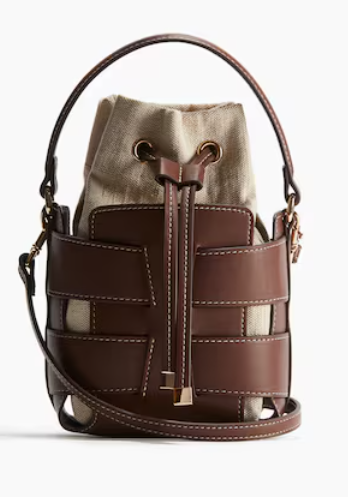
\includegraphics[width=\linewidth]{9a50dc75f5f24881ad0145747f79ff8d.png}};
\draw[white,rounded corners=\ClipSep,line width=\ClipSep]
      (current bounding box.north west) --
      (current bounding box.north east) --
      (current bounding box.south east) --
      (current bounding box.south west) -- cycle;
\end{tikzpicture}
\end{minipage}

\cvsection{Profil}
Data scientist passionné par la transformation de données complexes en solutions à forte valeur ajoutée, j’évolue aujourd’hui en CDI sur des projets d’IA de bout en bout. Mon parcours associe expertise technique (Machine / Deep Learning, NLP, ingénierie statistique) et sens du produit pour livrer des applications robustes et compréhensibles. Autonome et proactif, j’apprécie le travail en équipe et la veille technologique continue. Je recherche des environnements innovants où relever de nouveaux défis et contribuer à des projets ambitieux.

\cvsection{EXPÉRIENCE}

\colorbox{maincolor}{%
  \begin{minipage}{\linewidth}
    \textbf{Data Scientist \& Développeur IA} \\ Prepaya \\ Jan 2024 - Présent
    \begin{itemize}
      \item Conçu et déployé une plateforme IA full-stack (Python/Flask) sur Heroku, offrant un accès centralisé aux modèles pour les équipes métiers. \item Implémenté des algorithmes de Machine et Deep Learning (Scikit-learn, TensorFlow, Keras) pour l’analyse de séries chronologiques et la prédiction. \item Industrialisé le pipeline de données via API OpenAI, PostgreSQL et CI/CD GitHub, sécurisant la qualité et la traçabilité des livraisons.
    \end{itemize}
  \end{minipage}}

\vspace{3mm}


\colorbox{maincolor}{%
  \begin{minipage}{\linewidth}
    \textbf{Apprenti Risk Analyst \& Data Scientist} \\ AXA XL (Groupe AXA) \\ Déc 2022 - Déc 2023
    \begin{itemize}
      \item Automatisé la collecte des données financières avec Python/VBA, réduisant de 50 \% le temps de préparation des rapports. \item Créé des tableaux de bord Power BI et Excel pour la facturation, donnant une visibilité temps réel aux équipes Finance et Management. \item Développé un modèle de scoring sinistres prédictif, affinant la politique de risque et améliorant la prise de décision.
    \end{itemize}
  \end{minipage}}

\vspace{3mm}


\colorbox{maincolor}{%
  \begin{minipage}{\linewidth}
    \textbf{Apprenti Data Scientist} \\ Prepaya \\ Sep 2021 - Aoû 2022
    \begin{itemize}
      \item Implémenté des modèles NLP (T5, BERT, TopicRank) pour générer automatiquement des formulaires et accélérer la production de contenus. \item Réalisé une analyse de sentiments des commentaires clients, fournissant des insights exploitables au marketing. \item Automatisé la collecte de données web (BeautifulSoup, Selenium) et structuré le pipeline d’analyse sous Python.
    \end{itemize}
  \end{minipage}}

\cvsection{FORMATION}

    \begin{tabularx}{\linewidth}{@{}c X@{}}
    \textcolor{sidetext}{\faGraduationCap} &
    \textbf{Master 2 Data Science} \\
    & Sorbonne Université \\
    & \begin{itemize}[leftmargin=*]
  \item Analyse de données avancée, séries temporelles et modèles de structure latente. \item Machine Learning, Deep Learning et apprentissage statistique appliqués à des cas réels. \item Bases de données, calcul parallèle et projets de data engineering en environnement Big Data.
\end{itemize} \\
    & \textit{Sep 2021 - Mar 2022}
    \end{tabularx}
    

% --------- colonne droite (bleue) ---------------------------------
\switchcolumn\color{white}\hspace*{0.4cm}\begin{minipage}{0.88\linewidth}

\cvsection{CONTACT}
\begin{tabular}{@{}c l}
  \faPhone & \href{tel:0753481453}{0753481453} \\[2pt]
  \faEnvelope & \href{mailto:papesalioufall2@gmail.com}{papesalioufall2@gmail.com} \\[2pt]
  \faMapMarker & 95300 Pontoise\\ \\[2pt]
  \faLinkedin & \href{@pape-saliou-fall-43154a211/}{}
\end{tabular}

\cvsection{COMPÉTENCES}

\begin{itemize}[leftmargin=*]
\item Python
\item SQL
\item PowerBI
\item MachineLearning
\item DeepLearning
\item NLP
\item Git\end{itemize}
\par\bigskip 

\cvsection{LANGUES}
\begin{itemize}[leftmargin=*]
\item Français - \textcolor{gray}{Maternel}
\item Anglais - \textcolor{gray}{B2}\end{itemize}
\par\bigskip 
\cvsection{INTÉRÊTS}
\begin{itemize}[leftmargin=*]
\item Football
\item Natation
\item Lecture
\end{itemize}

\end{minipage}
\end{paracol}
\end{document}
